\chapter{Popis softvéru}\label{chap:popis}

V predchádzajúcich kapitolách sme si popísali niektoré dátové štruktúry a 
vybrané algoritmy. Hlavnou náplňou je ich vizualizácia. Ako sme povedali v 
úvode, vizualizácia je názorné vykreslenie dátovej štruktúry. Vizualizácia 
algoritmu je znázornenie priebehu algoritmu na dátovej štruktúre. 

\section{Analýza existujúcich riešení}

Softvér vizualizuje dátové štruktúry, algoritmy na nich a popisuje ako 
algoritmy fungujú. Preto sa hodí ako učebná pomôcka pre študentov na 
samoštúdium a pre učiteľov na názorné ukážky pri vyučovaní.

Vizualizované dátové štruktúry sú známe a rozšírenie vizualizácie je veľké, 
preto exituje veľa podobných aplikácií a appletov znázorňujúcich tieto 
dátové štruktúry a algoritmy. Väčšina z nich je na úrovni školských projektov 
a je súkromná. Preto porovnám len tie vizualizácie, ktoré sú vybrané skupinou 
ľudí venujúcej sa vizualizácií algoritmov; skupinou {\tt algoviz.org}. 
Analýza prebehla v máji 2012.

\subsection{Union/Find Algorithm Visualization (union-find)}\label{sec:ufav}
Tento malý applet je súčasťou väčšieho projektu \emph{Virginia Tech Algorithm 
Visualizations}. Applet je implementovaný v programovacom jazyku \Java\ a po
grafickej stránke je veľmi podobný ako zvyšok projektu. Softvér je vydaný pod 
licenciou {\tt GPL}. Vyvíjali ho Cris Kania a Cliff Shaffer počas jesene 2004. 

Je dostupný na: \url{http://research.cs.vt.edu/AVresearch/UF/}.

\subsubsection{Popis}
Applet poskytuje operácie $\union$ a $\find$ na ôsmich, dvanástich, šestnástich 
alebo dvadsiatich vrcholoch. Na obrázku \ref{img:vis:ufav} je obrazovka 
appletu. Môžeme vidieť, že dátová štruktúra je vykreslená vpravo. Použitý je 
jednoduchý algoritmus. Vpravo dole je vykreslená reprezentácia v poli a 
pre každý vrchol je vypísaný otec. Vľavo je riadne vypísaný zoznam vykonaných 
krokov, ktorý je navyše farebne odlíšený. Farby vo výpise a vo vizualizácií 
spolu korešpondujú. Vľavo dole sú nastavenia. 
Applet poskytuje operácie $\union$ s heuristikou na spájanie a $\find$ s 
možnosťami bez kompresie a s kompresiou cesty 
(popísané v sekciách \ref{sec:komp-union} a \ref{sec:komp-cesta}).

\begin{figure}
\centering
\greybox{%
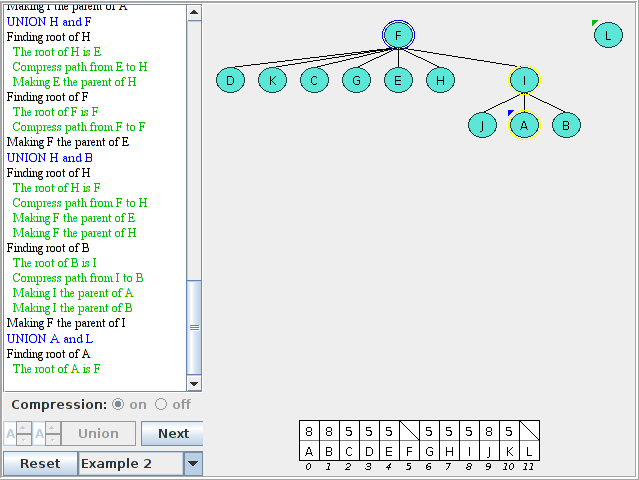
\includegraphics[scale=0.5]{obrazky/union-find-kania-shaffer-fall-2004}%
}
\caption{\emph{Softvér Union/Find Algorithm Visualization.} V ľavej časti 
obrazovky sa nachádzajú výpisy a možnosti nastavenia, vpravo je vizualizácia 
dátovej štruktúry a prebiehajúceho algoritmu.}
\label{img:vis:ufav}
\end{figure}

%\subsection{Hodnotenie}
Softvér poskytuje priestor len na malé príklady. Na 
pochopenie ako fungujú algoritmy to je postačujúce. Ovládanie je intuitívne.

\subsection{AlVie (union-find)}\label{sec:alvie}
% \citat{%
% The girl's name Alvie, also used as boy's name Alvie, is a variant of Alvina 
% (old English), and the meaning of Alvie is "elf or magical being, friend".}{%
% \url{http://alvie.algoritmica.org/alvie3/quickstart}}

AlVie je veľký projekt. Je to prostredie na vizualizáciu algoritmov, 
vytváranie vlastných vizualizácií a veľmi flexibilné pridávanie vlastného 
materiálu. Slúžil na podpru talianských škôl. Projekt momentálne spravuje 
Pilu Crescenzi. Je implementovaný v jazyku \Java.

\subsubsection{Popis}
Na webovej stránke projektu (\url{http://alvie.algoritmica.org/alvie3}) je 
prehľadný popis funkcionality a používania. Aplikácia ponúka množstvo 
nastavení a veľa možností exportovania danej vizualizácie. Avšak nepodarilo sa 
mi nastaviť si vlastný vstup, preto som ostal len pri základnej možnosti. 
Union-find je tu bohužiaľ implementovaný nie cez les, ale ako spájaný zoznam 
(obr. \ref{img:vis:alvie}), čo asymptoticky spomaľuje beh algoritmu.

\begin{figure}
\centering
\greybox{%
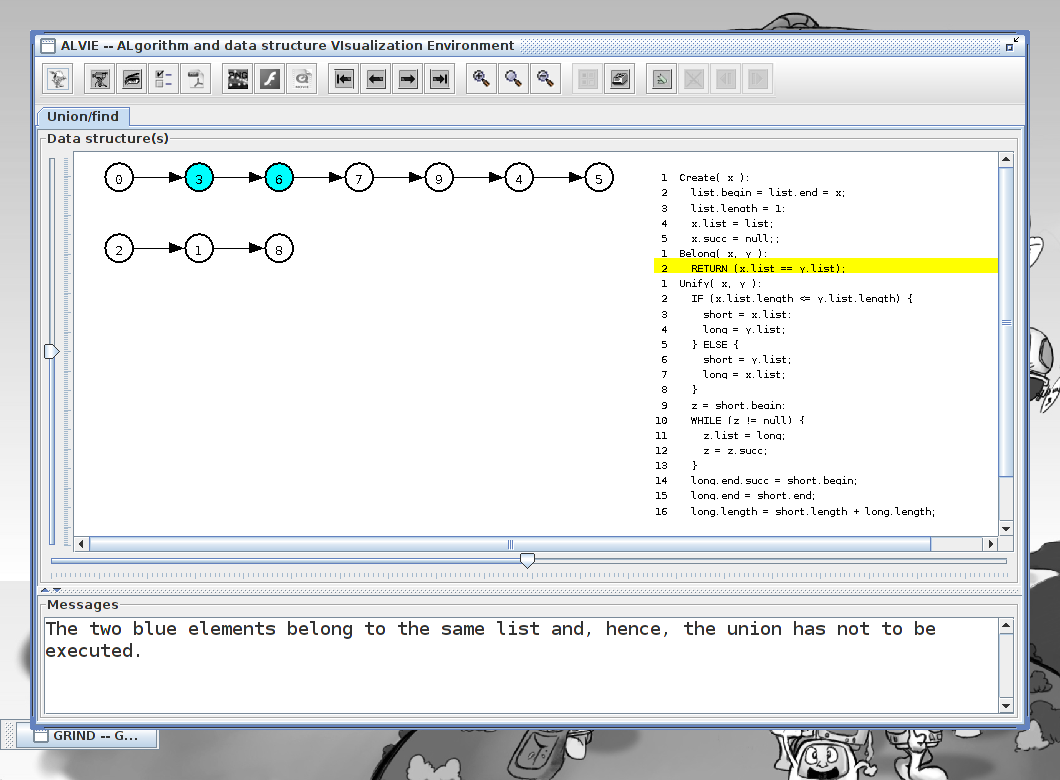
\includegraphics[scale=0.37]{obrazky/AlVie}%
}
\caption{\emph{Softvér Alvie.} Prebieha {\tt XML} skript. Vpravo je pomocný 
pseudokód.}
\label{img:vis:alvie}
\end{figure}

Napriek veľkému množstvu dodávaných algoritmov, nastavení a 
zobrazenému pseudokódu počas vizualizácie má tento softvér nevýhody v podobe 
horšieho ovládania a neoptimálnej implementácie disjunktných množín.

\subsection{Data Structure Visualizations (union-find)}\label{sec:galles}

Vizualizácia union-find algoritmu je v tomto prípade súčasťou veľkého projektu 
využívajúceho veľa technológií (Flash, \Java, {\tt HTML5}). Autorom je David 
Galles.

Projekt je prístupný na: 
\hbox{\url{http://www.cs.usfca.edu/~galles/visualization/}}.

\subsubsection{Popis}

Autor si dal záležať na použití moderných technológií a celá internetová 
aplikácia vyzerá veľmi pekne. Aplikácia zobrazuje štruktúru aj ako les aj ako 
pole. Dá sa nastaviť rýchlosť algoritmu a možnosti heuristík. Vstupné 
parametre operácií sa zadávajú cez textové políčka.

\begin{figure}
\centering
\greybox{%
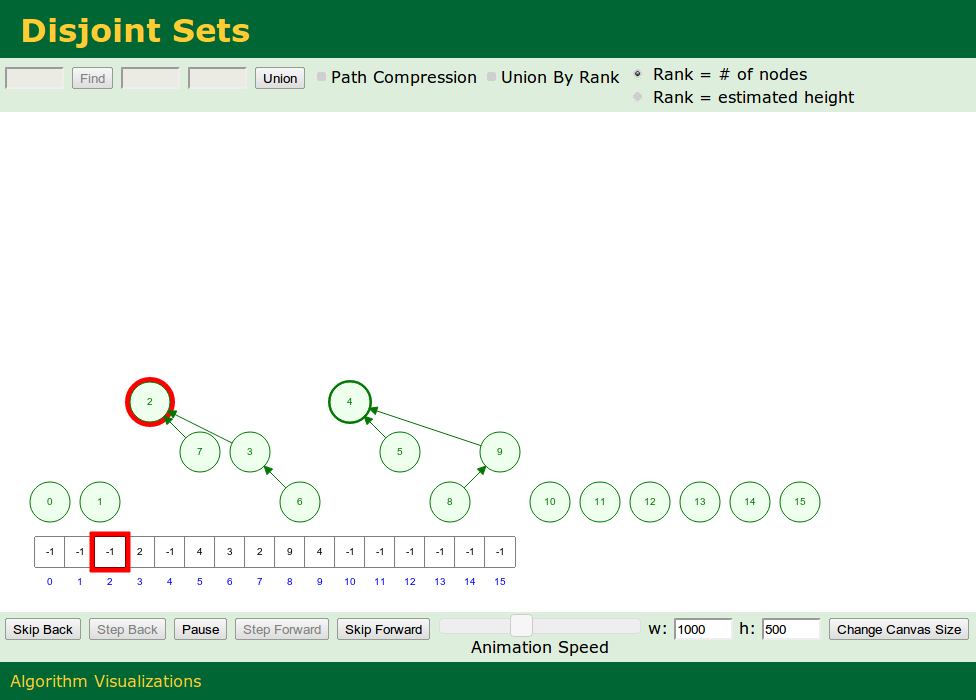
\includegraphics[scale=0.37]{obrazky/galles}%
}
\caption{\emph{Softvér Data Structure Visualizations.} Prebieha spájanie dvoch 
množín. Celá aplikácia beží v internetovom prehliadači.}
\label{img:vis:galles}
\end{figure}

Aplikácia je dobre popísaná, dá sa na nej nastaviť všetko potrebné vrátane 
rýchlosti premietania a veľkosti vykreľovacej plochy. Nevýhodou je, že 
nevypisuje, čo sa práve deje a teda používateľ musí algoritmus poznať.

\subsection{TRAKLA2 (trie)}\label{sec:trakla}

TRAKLA2 je učebná pomôcka vyvíjaná skupinou ľudí "Software visualization 
group". Všetci sú študenti alebo zamestnanci na Helsinskej technickej 
univerzite. Obsahuje veľa algoritmov a ku každému má sadu úloh, ktoré žiak 
môže riešiť. 

Celý výučbový systém je dostupný a popísaný na: 
\url{http://www.cse.hut.fi/en/research/SVG/TRAKLA2/index.shtml}.

\begin{figure}
\centering
\greybox{%
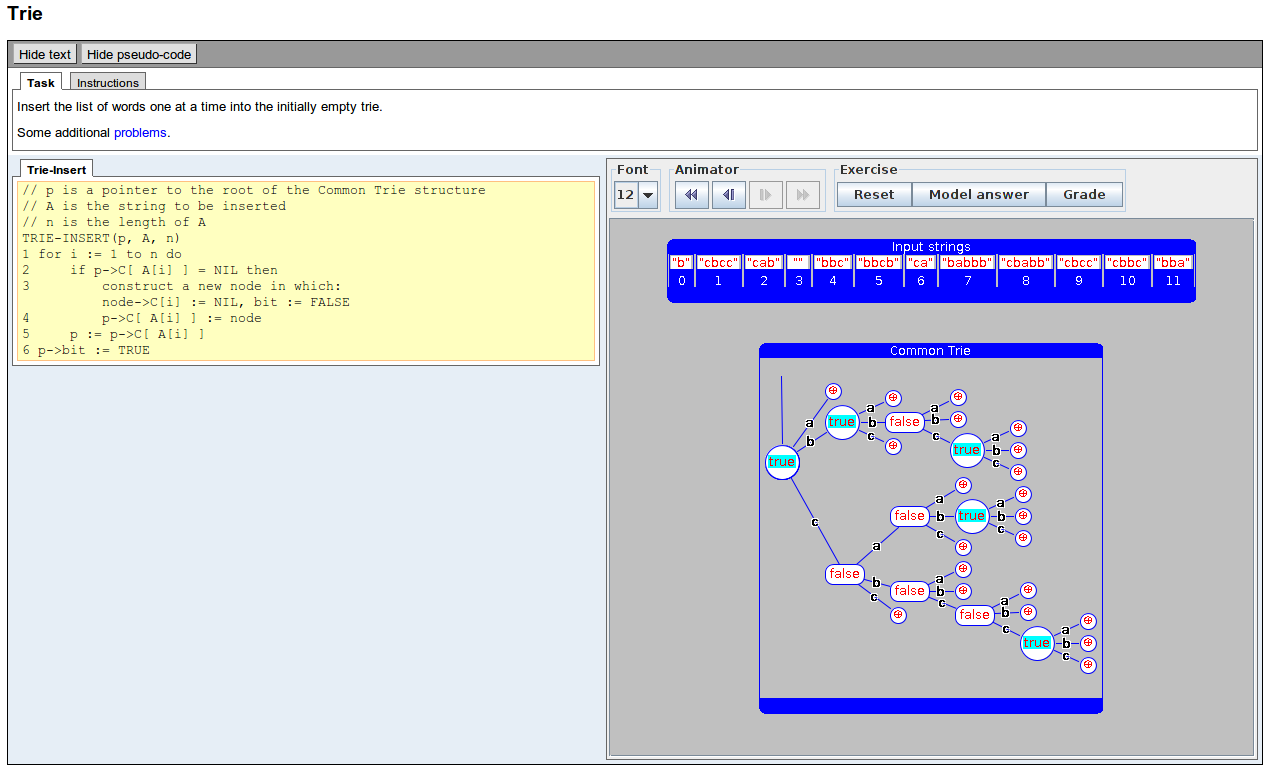
\includegraphics[scale=0.33]{obrazky/trakla2}%
}
\caption{\emph{Prostredie TRAKLA2.} Riešenie zadania; budovanie písmenkového 
stromu obsahujúceho zadané reťazce. Celá aplikácia beží v internetovom 
prehliadači.}
\label{img:vis:trakla2}
\end{figure}

\subsubsection{Popis}

Už na prvý pohľad je vidieť, že na projekte sa podieľa veľa ľudí. Stojí za ním 
viac ako 40 ľudí. Systém je premyslený, každý algoritmus obsahuje pseudokód. 
Všade sú pomôcky, takže ak sme niečomu nerozumeli, našli sme navigáciu na 
odpoveď. 

Samotné vizualizovanie písmenkového stromu je vykonávané niektorým tesným 
algoritmom, čo je veľká výnimka pri vizualizáciach, ktoré sa nezaoberajú tým, 
ako vykresľovať grafy! V hornej časti je umiestnený pomocný text, vľavo je 
pseudokód a vpravo je dátová štruktúra, na ktorej sa vykonáva zadanie (obrázok 
\ref{img:vis:trakla2}). Je možné zvoliť si veľkosť písma.

Všetko je spravené pekne a prehľadne, možno grafická stránka by sa dala 
vylepšiť. Jediná chyba, na ktorú som narazil bola, že pokiaľ som kroky 
nevykonával v správnom poradí, nebola mi uznaná správna odpoveď aj keď 
výsledok správny bol. Toto je ale špecifická chyba len pre písmenkový strom 
(pre iné dátové štruktúry môže poradie pridávania zmeniť reprezentáciu).

\subsection{Sufixové stromy}

Na sufixové stromy, konkrétne Ukkonenov algoritmus, ktorý sme vizualizovali, 
sa podarilo nájsť len jednu a aj to textovú vizualizáciu. 

\subsection{Ďalšie vizualizácie}

Uviedli sme tri softvéry pre union-find a jeden pre písmenkový 
strom. Na jednoduché 
písmenkové stromy sme viac vizualizácií nenašli. Ďalšie programy vizualizovali 
textové dáta alebo iné modifikácie písmenkových stromov (niektoré sú uvedené v 
sekcií \ref{sec:trie:pouzitie}).

Všetky aplikácie, ktoré sme analyzovali, však mali jeden spoločný nedostatok. 
Nedalo sa rýchlo dostať ku stavu, kedy je na štruktúre vykonaných veľa operácií 
a pokračovať z tohto stavu ďalej. Na prázdnej dátovej štruktúre nemusí byť 
dobre vidieť priebeh operácie. Taktiež to môže byť nepríjemné v prípade, že si 
chce používateľ len pripomenúť na už existujúcej štruktúre ako algoritmus 
funguje, prípadne ako štruktúra po vykonaných operáciách vyzerá.
% \todo{
% Cieľom tejto etapy je oboznámenie sa s prostredím, v ktorom bude aplikácia používaná. 
% Dôraz sa kladie na hlbšie pochopenie interakcie aplikácie s prostredím. 
% Ak existujú, treba vykonať aj analýzu podobných systémov.
% }

\clearpage
\section{Špecifikácia požiadaviek}

Počas analýzy sme zistili, že vizualizácie mali nedostatky najmä v tom, že sa 
na nich nedalo naraz vykonať viac operácií. V prípade, že sa dalo (sekcia 
\ref{sec:alvie}), tak sa z tohto stavu nedalo pokračovať. Ďalej sme zistili, 
že aplikácie neposkytujú rozšírené metódy vstupu. Všeobecne bolo veľmi 
obtiažne vôbec vybudovať väčšiu dátovú štruktúru, na ktorej by boli algoritmy 
a hlavne ich efektivita viditeľnejšia. Pri niektorých vizualizáciach nebolo 
jasne viditeľné, čo sa ide vykonať.

\subsection{Požiadavky}

Naša aplikácia bude používaná najmä študentmi, ktorí si chcú zopakovať učivo 
z prednášok, alebo učiteľmi, ktorí túto aplikáciu budú chcieť využívať na 
hodinách.

Preto sa nám zdalo byť vhodné, aby študent dostával výpisy o tom, čo sa bude 
diať a aby bolo prostredie pre študenta dostatočne používateľsky príjmené. Pre 
učiteľa je potrebné, aby sa aplikácia prijateľne zobrazovala cez projektor, 
aby bola dátová štruktúra od začiatku naplnená (veľakrát sa algoritmy 
vysvetlujú na pripravenej dátovej štruktúre) a taktiež, aby bolo prostredie 
používateľsky príjemné.

Softvér ako taký mal vizualizovať tieto veci:
\begin{itemize}
\item dátovú štruktúru pre disjunktné množiny reprezentovanú stromom a na nej 
tieto algoritmy:
	\begin{itemize}
	\item naivné spájanie, spájanie podľa ranku;
	\item nekomprimované hľadanie, hľadanie s jednoduchou kompresiou, hľadanie s 
	delením cesty, hľadanie s pólením cesty.
	\end{itemize}
\item písmenkový strom (trie) a na ňom tieto algoritmy:
	\begin{itemize}
	\item vkladanie slova;
	\item testovanie na prítomnosť slova;
	\item mazanie slova.
	\end{itemize}
\item sufixový strom a jeho vytváranie pomocou Ukkonenovho algoritmu.
\end{itemize}

\subsection{Prevádzkové požiadavky}

Pretože ľudia používajú rôzne operačné systémy a softvér nepracuje so 
špecifickými systémovými zdrojmi bolo potrebné, aby bola aplikácia nezávislá 
od operačného systému. Keďže má byť dostupná na študentské účely, nemala by 
byť hardvérovo náročná.
% \todo{
% Východiskom tejto etapy je etapa analýzy. 
% Zaoberá sa úlohami, ktoré má aplikácia zabezpečiť. 
% Oboznámime sa s prostredím, v ktorom bude aplikácia používaná. 
% Zaujímame sa o to, čo chce zadávateľ riešiť, čo požaduje, aby aplikácia vykonávala a pre koho je určená. 
% Zatiaľ nás nezaujíma spôsob realizácie.  
% Cieľom špecifikácie požiadaviek je stanovenie služieb, ktoré zákazník požaduje od systému a ohraničenia na jeho vývoj a prevádzku. 
% Teda zaujímame sa o funkcionálnu stránku systému, potom o to, aké by mali byť vstupy a výstupy systému 
% a s akými údajmi systém bude pracovať, potom o prevádzkové požiadavky 
% (počet a charakteristika používateľov, časová odozva systému, potrebný hardvér a softvér, bezpečnosť a ochrana systému a iné potrebné požiadavky). 
% Prevádzkové požiadavky nazývame aj nefunkcionálne požiadavky. 
% Detailný opis špecifikácie požiadaviek na softvér  najdeme v (1) alebo v štandarde IEEE 830.
% }

\section{Návrh}

Táto práca je pokračovaním práce Jakuba Kováča a preto návrh vychádzal hlavne z 
jeho práce. Našou hlavnou úlohou bolo implementovať vybrané dátové štruktúry a 
algoritmy. V~nasledujúcich častiach sme popísali požiadavky kladené na náš 
softvér, či už z hľadiska technického alebo používateľského, zvolené 
technológie a rozhranie systému.
% vzťahy medzi časťami softvéru, 
%štruktúru dát a rozhranie systému.

\subsection{Technické požiadavky}

Softvér slúži na vizualizáciu a bolo potrebné ho implementovať multiplatformovo.
Taktiež slúži aj na opisovanie prebiehajúceho algoritmu, teda 
bola potrebná plocha na vykresľovanie, plocha na vypisovanie toho, čo sa deje, 
ovládacie prvky algoritmu a ovládacie prvky na výber dátových štruktúr.

\subsection{Používateľské požiadavky}

Ako sme už naznačili, používateľmi sú prevažne študenti a učitelia, veľmi 
pravdepodobne informatiky. Preto bolo vhodné okrem obyčajného a pomalšieho 
zadávania vstupu po jednej operácií vytvoriť prostredie, v ktorom sa bude dať 
zadávať aj zložitejší vstup.

Ďalej bolo potrebné názorne vizualizovať dátové štruktúry a všetko podstatné k 
pochopeniu algoritmov. Konkrétne pri union-finde išlo o prípadné ranky, 
pri písmenkovom strome o odstraňovanie vetiev, prehľadné vykresľovanie pri 
prebiehajúcich algoritmoch a pri sufixovom strome sufixové linky, práve 
pridávaný sufix a celé slovo, ktorému sufixový strom budujeme.

\subsection{Použité technológie}

Keďže projekt bol pokračovaním predošlej práce za hlavný programovací jazyk 
bola zvolená \Java. Na grafické znázornenie sú to jednotlivé triedy balíkov 
AWT a Swing. Na generovanie náhodných reťazcov sme použili špeciálne upravenú 
triedu s návrhovým vzorom \emph{singleton}. Vďaka celkovej nenáročnosti na 
technológie a zameraniu projektu nebolo potrebné použiť viac technológií.

\subsection{Rozhranie aplikácie}

Rozhranie vizualizácií bolo podobné ako všetkých iných štruktúr 
implementovaných v predošlej verzií softvéru. Vstupné dáta boli zadávané do 
vstupného textového poľa, alebo klikaním myšou. Podľa stlačeného tlačidla sa 
spustil daný proces. Výstupne údaje boli prezentované vo vykresľovacom okne 
pre dátovú štruktúru a vo výpise pre komentáre. Vykreslená štruktúra sa dala 
zväčšiť, zmenšiť a posunúť pomocou myšky.

Pre každú dátovu štruktúru bolo potrebné zabezpečiť vstupné textové pole, 
prípadne dodatočné vstupné metódy a tlačidlá pre všetky operácie.

\subsubsection{Union-find}

Pre union-find bolo potrebné zabezpečiť vstupné textové pole, tlačidlá pre 
operácie $\union$ a $\find$, vyberanie vstupných prvkov myšou, možnosť výberu 
medzi naivným spájaním a spájaním podľa ranku a medzi hľadaním zástupcu bez 
kompresie, s jednoduchou kompresiou, delením cesty a pólením cesty (popísané 
v kapitole \ref{chap:uf}).

\subsubsection{Písmenkový strom}

Pri písmenkovom strome bolo nutné zabezpečiť vstupné pole tak, aby sa do systému 
dostali slová, len s abecedou, ktorú chceme. Pre nás abecedu tvorili veľké 
písmená anglickej abecedy. Ďalej bolo potrebné, aby sa dal pridať do stromu 
ucelenejší text. Na vykonávanie operácií $\put$, $\find$ a $\delete$ bolo 
potrebné implementovať tlačidlá.

\subsubsection{Sufixový strom}

Sufixový strom bolo potrebné vytvoriť zo vstupného slova. Preto treba na tento 
účel implementovať jedno tlačidlo.

\subsection{Prepojenie s predošlým systémom}

Po implementácií mal systém tvoriť jeden celok, preto bola potreba dbať na 
celistvosť a podobný štýl programovania. Na jednotlivé implementovanie 
obrazoviek, vstupných polí a tlačidiel bolo nutné použiť už existujúce 
rozhranie a tak isto na implementáciu vizualizácie bolo treba použiť rovnaký 
systém, ktorý vyžadoval dedenie z predpripravených abstraktných tried. 

V hornej lište aplikácie bolo menu na výber dátových štruktúr a menu 
na výber jazyka. Systém fungoval na princípe kontajnera inštanciovaných tried 
udržiavajúcich jednotlivé obrazovky. Objekty mali priradenú dátovú štruktúru. 
Panel obsahoval plochy pre vykresľovanie, výpis komentárov (toho, čo sa bude 
diať) a ovládacie tlačidlá. Pri vykonaní zvolenej operácie sa spustilo nové 
vlákno vykonávajúce danú operáciu a obsluhujúcu obrazovku.

Všetky predošlé vizualizácie pracovali s binárnymi stromami. Naše dátové 
štruktúry však boli všeobecné stromy, respektíve lesy. Preto bolo nutné 
implementovať triedu na prácu so všeobecnými stromami.
% \todo{
% V tejto etape sa ujasňuje koncepcia systému. 
% Navrhne sa jeho dekompozícia, určia sa vzťahy medzi časťami systému a ohraničenia funkcionality. 
% Túto časť návrhu zvyčajne modelujeme technikami softvérového inžinierstva napr. procesným modelom DFD (Data Flow Diagram, str.24 v (1)) 
% Dekompozícia sa môže urobiť aj na základe iných princípov ako je funkcionálny (str. 53 v (1)). 
% V ďalšom sa identifikuje štruktúra údajov, ktoré do systému vstupujú, ktoré systém spracováva a produkuje. 
% Vzťah medzi údajmi sa modeluje entitno-relačným diagramom, v ktorom sa pomenovávajú vzťahy medzi údajovými entitami. 
% Ak použijeme model DMD (Data Model Diagram), potom v ňom znázorňujeme kvantifikované vzťahy dohodnutými značkami na označenie kardinality. 
% Ak rozložíme vzťah typu M:N pomocou väzobnej entity, potom dostávame fyzický model údajov.  (str.31 v (1))
% V etape návrhu sa navrhne rozhranie systému ( čo do systému vstupuje a čo z neho vystupuje), 
% navrhne sa typ používateľského rozhrania (príkazovo orientované rozhranie, menu, priame riadenie, komunikácia v prirodzenom jazyku ), 
% plán realizácie systému a stanovia sa podmienky, za akých bude používateľ akceptovať produkt. 
% Odhadnú sa potrebné ľudské a materiálne zdroje a navrhne sa postup zaškolovania používateľov.
% }

